\documentclass{article}
\usepackage[utf8]{inputenc}
\usepackage{amsmath}
\usepackage{amssymb}
\usepackage{amsthm}
\usepackage{tikz}
\setlength{\parindent}{0pt}

\newtheorem*{theorem}{Theorem}
\newtheorem*{definition}{Definition}
\newtheorem*{lemma}{Lemma}
\newtheorem*{corollary}{Corollary}
\newtheorem{example}{Example}

\title{Lecture 8: Partial Derivatives}
\author{}
\date{}

\begin{document}
    
\maketitle

\section{Multivariable Functions}

Multivariable functions are functions whose values depend on more than one 
independent variables.

Examples of Multivariable functions:
\begin{itemize}
  \item $f(x, y) = x^2 + y^2$
  \item $f(x, y) = \frac{1}{x + y},\, x + y \neq 0$
  \item $f(x, y) = \frac{1}{\sqrt{y}},\, y > 0$
  \item The temperature of a certain point on earth at a given time is a 
  multivariable function of latitude, longitude, and height.
\end{itemize}

For simplicity, in this course we will mainly study multivariable functions with 
two or three variables, but the concepts apply to any multivariable functions 
with any number of variables.

\section{Visualization of Multivariable Functions with Two Variables}

\subsection{Function Graph}

For a single-variable function $f$, we plot the function graph as $(x, f(x))$, 
which is very straightforward.

For a multivariable function with two variables $f$, we can similarly plot the 
function graph as $(x, y, f(x, y))$, which is a surface in 3D space.

\begin{example}
  Plot the graph of the function $f(x, y) = -y$.

  The equation of the function graph is $z = -y$, which is a plane.
\end{example}

\begin{example}
  Plot the graph of the function $f(x, y) = 1 - x^2 - y^2$.

  The equation of the function graph is $z = 1 - x^2 - y^2$, whose shape is not 
  so easy to be identified. \\
  We can first take a look at the intersection between the function graph and 
  the $x-z$ plane, which means let $y = 0$. Hence, the equation of the 
  intersection is $z = 1 - x^2$, which is a parabola. \\
  We can then take a look at the intersection between the function graph and the 
  $y-z$ plane, which means let $x = 0$. Hence, the equation of the intersection
  is $z = 1 - y^2$, which is a parabola. \\
  Finally, we can take a look at the intersection between the function graph and 
  the $x-y$ plane, which means let $z = 0$. Hence the equation of the 
  intersection is $x^2 + y^2 = 1$, which is a unit circle. \\
  Based on the above information, we can guess the shape of the function graph 
  is as follows:
\end{example}

From the above examples, we can see that the graph of multivariable functions 
with two variables are not only hard to plot, but also often hard to read.

\subsection{Contour Plot}

Contour Plot is another way to visualize multivariable functions with two 
variables. It basically shows all the points where $f(x, y) =$ some fixed 
constants, which are chosen at regular intervals. Examples include contour map,
isotherm map, etc.

From geometric point of view, contour plot is equivalent to using horizontal 
planes ($z =$ some fixed constants) to slice the function graph and combining 
the intersection points in the $x-y$ plane.

\begin{example}
  Find the contour plot of the function $f(x, y) = -y$.
  
  \begin{tikzpicture}
    \draw[->] (-3, 0, 0) -- (3, 0, 0) node[below right] {x};
    \draw[->] (0, -3, 0) -- (0, 3, 0) node[right] {y};
    \draw (0, 0) node[below right] {O};
    \draw (3, 0) node[above right] {0};
    \draw[-] (-2.5, -1, 0) -- (2.5, -1, 0) node[right] {1};
    \draw[-] (-2.5, 1, 0) -- (2.5, 1, 0) node[right] {-1};
    \draw[-] (-2.5, -2, 0) -- (2.5, -2, 0) node[right] {2};
    \draw[-] (-2.5, 2, 0) -- (2.5, 2, 0) node[right] {-2};
  \end{tikzpicture}

\end{example}

\begin{example}
  Find the contour plot of the function $f(x, y) = 1 - x^2 - y^2$.

  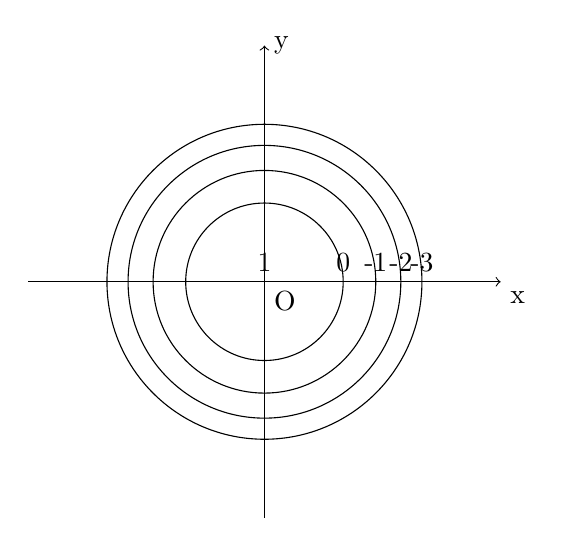
\begin{tikzpicture}
    \draw[->] (-3, 0, 0) -- (3, 0, 0) node[below right] {x};
    \draw[->] (0, -3, 0) -- (0, 3, 0) node[right] {y};
    \draw (0, 0) node[below right] {O};
    \draw (0, 0) node[above] {1};
    \draw (0, 0) circle (1);
    \draw (1, 0) node[above] {0};
    \draw (0, 0) circle (1.414);
    \draw (1.414, 0) node[above] {-1};
    \draw (0, 0) circle (1.732);
    \draw (1.732, 0) node[above] {-2};
    \draw (0, 0) circle (2);
    \draw (2, 0) node[above] {-3};
  \end{tikzpicture}

  Notice that the distance between two adjacent contour lines becomes smaller 
  going outwards, which means the slope becomes larger in that direction.

\end{example}

\section{Partial Derivatives}

For single-variable functions, we have derivatives to describe the rate of 
change of the function value with the independent variable.

How do we do the same for multivariable functions, which have more than one 
independent variables? We can assume that only one independent variable in a 
multivariable function can change, i.e. treating other independent variables as 
constants, in this way we can adapt the definition of derivatives from 
single-variable functions to multivariable functions. Such derivatives are 
called \textbf{Partial Derivatives}. The notation of partial derivatives is 
$\frac{\partial f}{\partial x}$, where the symbol $\partial$ is read as 
\emph{partial}, and the independent variable in the denominator is called the 
\emph{partial variable}, which is the variable that can change, or is not 
treated as a constant. In applied mathematics, the notation of partial 
derivatives can also be $f_x$.

\subsection{Definition of Partial Derivatives}

\begin{gather*}
  \frac{\partial f}{\partial x}(x_0, y_0) = \lim_{\Delta x \to 0}\frac{f(x_0 + \Delta x, y_0) - f(x_0, y_0)}{\Delta x} \\
  \frac{\partial f}{\partial y}(x_0, y_0) = \lim_{\Delta y \to 0}\frac{f(x_0, y_0 + \Delta y) - f(x_0, y_0)}{\Delta y} \\
\end{gather*}

\subsection{Geometric Interpretation of Partial Derivatives}

A partial derivative of a multivariable function can be viewed as extracting a 
2D slice out of the plot of the function, and using the partial derivative to 
describe the slope of the tangent line in that slice.

\subsection{Computation of Partial Derivatives}

Since the definition of partial derivatives is the same as the derivative of 
single-variable functions, so the formulas with the derivative of 
single-variable functions also apply to partial derivatives. In the computation, 
we just need to treat other variables as constants and apply the proper 
derivative formulas.

\bigskip

Reason why formulas of the derivative of single-variable functions also apply to 
partial derivatives: \\
According to the definition of partial derivatives,
\begin{equation*}
  \frac{\partial f}{\partial x}(x_0, y_0) = \lim_{\Delta x \to 0}\frac{f(x_0 + \Delta x, y_0) - f(x_0, y_0)}{\Delta x}
\end{equation*}
Since $y_0$ doesn't change in the computation, we can ignore it in the formula 
just as ignoring other constant terms and factors in the function. Therefore,
\begin{equation*}
\begin{split}
  \frac{\partial f}{\partial x}(x_0, y_0) &= \lim_{\Delta x \to 0}\frac{f(x_0 + \Delta x, y_0) - f(x_0, y_0)}{\Delta x} \\
                                          &= \lim_{\Delta x \to 0}\frac{f(x_0 + \Delta x) - f(x_0)}{\Delta x} \\
\end{split}
\end{equation*}
which is the definition of the derivative of single-variable functions. 
Therefore, we can apply formulas of the derivative of single-variable functions 
to compute partial derivatives with treating other independent variables as 
constants.

\begin{example}
  Find the partial derivatives regarding $x$ and $y$ of the function 
  $f(x, y) = x^3y + y^2$.

  Solution:

  \begin{gather*}
    \frac{\partial f}{\partial x} = 3yx^2 \\
    \frac{\partial f}{\partial y} = x^3 + 2y \\
  \end{gather*}
\end{example}

\end{document}